\section{\label{sec:intro}Introduction}
In todays applications, data is continuously produced in various spots
ranging from network traffic, log file data, monitoring of
manufacturing processes or scientific experiments. The applications
typically emit data in non-terminating data streams at a high rate,
which poses tight challenges on the analysis of such streams.

We illustrate this by projects of our Collaborative Research Center
SFB-876. A first example is given by the FACT telescope that is
associated to project C3. This telscope observes cosmic showers by
tracking light that is produced by these showers in the atmosphere
with a camera.  These showers last about 20 nanoseconds and are
recorded with a camera of 1440 pixels at a sampling rate of 2 GHz. As
about 60 of these showers are currently recorded each second, a
5-minute recording interval quickly produces several gigabytes of raw
data.

Other high-volume data is produced in monitoring system behavior, as
performed in project A1. Here, operating systems are monitored by
recording fine grained logs of system calls to catch typical usage of
the system and optimize its resource utilization (e.g. for energy
saving). System calls occur at a high rate and recording produces a
plethora of log entries.

The project B3 focuses on monitoring (distributed) sensors in an
automated manufacturing process. These sensors emit detailed
information of the oven heat or milling pressure of steel production
and are recorded at fine grained time intervals. Analysis of this data
focuses on supervision and optimization of the production process.

\subsubsection*{From Batches to Streams}
The traditional batch data processing aims at computations on fixed
chunks of data in one or more passes. The results of these
computations again form a fixed outcome that can further be used as
input. A simple example is given by the computation of a prediction
model based on some fixed training set. After the determination of a
final model, the learning step is finished and the model is applied to
deliver predictions based on the learning phase. Similar situations
arise for the computation of statistics, creation of histograms, plots
and the like. From a machine learning perspective, this has been the
predominant approach of the last years.

Two aspects have been changed in the data we are facing today, which
requires a paradigm shift: The size of data sets has grown to amounts
intractable by existing batch approaches, and the rate at which data
changes demands for short-term reactions to data drifts and updates of
the models.

%\subsubsection*{Processing Masses of Data}
The problem of big data has generally been addressed by massive
parallelism. With the drop of hardware prizes and evolving use of
large cloud setups, computing farms are deployed to handle data at a
large scale. Though parallelism and concepts for cluster computing
have been studied for long, their applicability was mostly limited to
specific use cases.

One of the most influential works to use computing clusters in data
analysis is probably Google's revival of the {\em map-and-reduce}
paradigm \cite{googleMapReduce}. The concept has been around in
functional programming for years and has now been transported to
large-scale cluster systems consisting of thousands of compute
nodes. Apache's open-source {\em Hadoop} implementation of a
map-and-reduce platform nowadays builds a foundation for various
large-scale systems.

With the revival of map-and-reduce, various machine learning algorithms
have been proven to be adjustable to this new (old) way of computing.

%In the massive parallel settings, we are given a large set of examples
%$\mathbf{X} \subseteq \mathbb{R}^p$. Models on this data are typically
%computed by partitioning the data, computing intermediate results
%({\em map} phase) and merging these results to a final output ({\em
%  reduce} phase) as shown in Figure \ref{fig:mapReduce}.
%
%\begin{figure}[ht!]
%  \begin{center}
%        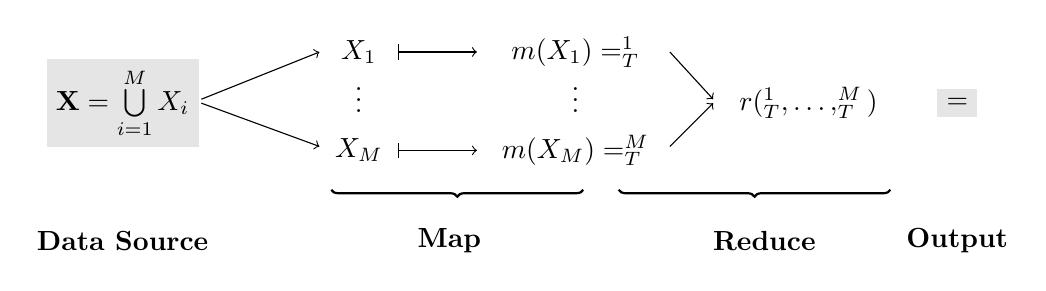
\begin{tikzpicture}
      \draw (-2.5,0.35) node[rectangle,fill=black!10] { $\mathbf{X} = \bigcup\limits_{i=1}^M X_i$ };
      \draw (-2.5,-1.4) node {\textbf{Data Source}};

      \draw[->] (-1.5,0.4) -- (0,1);
      \draw[->] (-1.5,0.35) -- (0,-0.2);

      \draw (0.5,1) node[rectangle] {$X_1$};
      \draw (0.5,-0.25) node[rectangle] {$X_M$};

      \draw (0.5,0.5) node {$\vdots$};


      \draw[|->] (1,1) -- (2,1);
      %\draw (1.5,1.25) node {$m$};
      \draw (3.25,1) node {$m(X_1) = \barw_T^1$}; %X_1'

      \draw[|->] (1,-0.25) -- (2,-0.25);
      %\draw (1.5,0) node {$m$};
      \draw (3.25,-0.25) node {$m(X_M) = \barw_T^M$}; %X_M'

      \draw (3.25,0.5) node {$\vdots$};

      %\draw (2,-0.25) node[rectangle,draw=black] {$m(X_M)$};

      \draw[->] (4.45,1) -- (5,0.4);
      \draw[->] (4.45,-0.2) -- (5,0.35);

      %\draw (6.21,0.35) node {$r(X_1',\ldots,X_M')$};
      \draw (6.21,0.35) node {$r(\barw_T^1,\ldots,\barw_T^M)$};

      \draw[decorate,decoration={brace, mirror},thick] (0.15,-0.75) -- (3.35,-0.75); % node at (6.5,-.5) {}; 
      \draw (1.65,-1.4) node {\textbf{Map}};

      \draw[decorate,decoration={brace, mirror},thick] (3.8,-0.75) -- (7.25,-0.75); % node at (6.5,-.5) {}; 
      \draw (5.65,-1.4) node {\textbf{Reduce}};

      \draw (8.1,0.35) node[rectangle,fill=black!10] {$=\barbarw$}; %$\ \overline{w}$.
      \draw (8.1,-1.4) node {\textbf{Output}};

    \end{tikzpicture}

%    \caption{\label{fig:mapReduce}The map-and-reduce paradigm.}
%  \end{center}
%\end{figure}


%%
%% Beispiele fuer Lerner die Map&Reduce fähig sind
%%  - Ensemble,...
%%  -
%% Software: Mahout,... andere?
%%

\subsection*{The Problem of Continuous Data}
Whereas the massive parallelism addresses the batch computation of
large volumes of data, it still requires substantial processing time
to re-compute prediction models, statistics or indexes once data has
been changed. Therefore it does not fully reflect the demands for
reacting to short-term drifts of data.

Within this work we will refer to this as the setting of {\em
  continuous data}, i.e. we consider an unbound source $D$ of data
that continuously emits data items $d_i$. In the following, we model
that data stream as a sequence
$$D = \langle d_0,d_1,\ldots,d_i,\ldots \rangle$$
with $i\rightarrow\infty$. The framing to operate on streaming data is
generally given by the following constraints/requirements:
\begin{itemize}
  \defitem{C1} continuously processing {\em single items} or {\em small batches} of data,
  \defitem{C2} using only a {\em single pass} over the data,
  \defitem{C3} using {\em limited resources} (memory, time),
  \defitem{C4} provide {\em anytime services} (models, statistics).
\end{itemize}


To catch up with the reqirements of large scale and continuous data,
online algorithms have recently received a lot of attention. The focus
of these algorithms is to provide approximate results while limiting
the memory and time resources required for computation. 
%The
%constraints for the data stream setting are generally defined by
%allowing only a single pass over the data, and focusing on
%approximation schemes to deal with the inbalance of data volume to
%computing resources. In addition, models computed on streaming data
%are expected to be queriable at any time.


\subsubsection*{Analysis of Continuous Data}
{\bf TODO: \"{U}berleitungssatz?}
Traditional data analysis methods focus on processing fixed size
batches of data and often require the data (or large portions of it)
to be available in main memory. This renders most approaches useless
for continuously analyzing data that arrives in steady streams. Even
procedures like preprocessing or feature extraction can quickly become
challenging for continuous data, especially when only limited
resources with respect to memory or computing power are available.

At any time $t$ we want to provide some model that reflects the
analysis of the items $d_i$ with $i\le t$.  Typical tasks to compute
on $S$ are
\begin{itemize}
\item Given $d_i \in \mathbb{N}$ - finding the top-$k$ most frequent
  values observed until $t$.
\item For $d_i \in \mathbb{N}^p$ - find the item sets $I \subset
  \mathbb{N}^p$ which most frequently occurred in the $d_i$.
\item With $d_i \subset X$, provide a classifier $c:X \rightarrow Y$,
  that best approximates the real distribution of labeled data $X
  \times Y$ (classification).
\item Provide a clustering $C$ for the data item $d_i$ observed so far (clustering).
\item Find indications on when the overall distribution of the $d_i$
  changes within the stream (concept drift detection).
\end{itemize}
Often, these tasks are further refined to models that focus on a
recent sliding window of the last $w$ data items observed, e.g. we are
interested in the top-$k$ elments of the last 5 minutes. 

Algorithms for solving these tasks on static data sets
exists. However, the challenging requirements in the continuous data
setting are the tight limits on the resources available for
computation. This can for example be realtime constraints, such as a
fixed limit on the time available for processing a data item, or a
bound on the memory available for computation.

Various algorithms have been proposed dedicated to computational
problems on data streams. Examples include online quantile computation
\cite{Greenwald/Khanna/2001a,Arasu/Manku/2004a}, distinct counting of
elements, frequent itemset mining
\cite{Charikar02findingfrequent,goethals2007,Cheng06maintainingfrequent},
clustering \cite{sohler2010,Aggarwal:2003} or training of classifiers
on a stream \cite{Domingos/Hulten/2000a}.

Here, we want to provide an abstract framework for putting online
learning algorithms to good use on data streams.

\subsection{Designing Stream Processes}

%\subsection*{Existing Frameworks}
%Various frameworks exist that support either of these two processing
%modes.
Parallel batch processing is addressing the setting of fixed data and
is of limited use if data is non-stationary but continuously produced,
for example in monitoring applications (server log files, sensor
networks).  A framework that provides online analysis is the MOA
library \cite{moa}, which is a Java library closely related to the
WEKA data mining framework \cite{weka}. MOA provides a collection of
online learning algorithms with a focus on evaluation and
benchmarking.

Aiming at processing high-volume data streams two environments have
been proposed by Yahoo! and Twitter. Yahoo!'s {\em S4} \cite{s4io}
as well as Twitter's {\em Storm} \cite{storm} framework do provide
online processing and storage on large cluster infrastructures, but
these do not include any online learning.

In contrast to these frameworks, the \streams library focuses on
defining a simple abstraction layer that allows for the definition of
stream processes which can be mapped to different backend
infrastructures (such as {\em S4} or {\em Storm}).

\subsubsection*{Our Contributions}
In this work we introduce the \streams library, a small software
framework that provides an abstract modelling of stream processes. The
objective of this framework is to establish a layer of abstraction
that allows for defining stream processes at a high level, while
providing the glue to connect various existing libraries such as MOA
\cite{moa}, WEKA \cite{weka} or the RapidMiner tool.

The set of existing online algorithms provides a valuable collection
of algorithms, ideas and techniques to build upon. Based on these core
elements we seek to design a process environment for implementing
stream processes by combining implementations of existing online
algorithms, online feature extraction methods and other preprocessing
elements.
%or implement and evaluate custom online algorithms 

Moreover it provides a simple programming API to implement and
integrate custom data processors into the designed stream processes.
The level of abstraction of this programming API is intended to
flawlessly integrate into existing runtime environments like {\em
  Storm} or the RapidMiner platform \cite{rapidminer}.

Our proposed framework supports
\begin{enumerate}
\item Modelling of continuous stream processes, following the {\em
    single-pass} paradigm,
\item Anytime access to services that are provided by the modeled
  processes and the online algorithms deployed in the process setup,
  and
\item Processing of large data sets using limited memory resources
\item A simple environment to implement custom stream processors and
  integrate these into the modelling
\item A collection of online algorithms for counting and classification
\item Incorporation of various existing libraries (e.g. MOA
  \cite{moa}) into the modeled process.
\end{enumerate}

The rest of this report is structured as follows: In Section
\ref{sec:relatedWork} we review the problem setting and give an
overview of related work and existing frameworks.
%% introduce some of the main objectives in data
%stream mining and provide some example use cases. 
Based on this we derive some basic building blocks for a modeling data
stream processes (Section \ref{sec:abstraction}). In Section
\ref{sec:processDesign} we present the XML based definition language
and several addition concepts that allow for designing stream
processes within the framework. Based on this we outline two example
use-cases for processing and analyzing streaming data with the
\streams library. Finally we summarize the ideas behind the \streams
library and give an outlook on future work. A comprehensive
description of the implementations and guides for setting up a
standalone processing environment provided by our framework is given
in the appendix.
